\documentclass{article}
\usepackage{hyperref}
\usepackage{enumitem}
\usepackage{graphicx}

\begin{document}
\title{Technical Paper Proposal: \\ Placement Algorithms for Heterogenous FPGAs}
\author{Brian Cheng \\ Department of Electrical and Computer Engineering}


\date{}
\maketitle

\section{Proposal}



\section{Abbreviations}
\begin{itemize}[label={--}, left=0.25cm] % Adjust label and left indent as desired
    \item FPGA: Field Programmable Gate Array
    \item VLSI: Very Large Scale Integration
    \item EDA: Electronic Design Automation
    \item VHSIC: Very High Speed Integrated Circuits
    \item HDL: Hardware Description Language
    \item VHDL: VHSIC HDL
    \item HLS: High Level Synthesis
    \item PL-PS: Programmable Logic - Processing System
    \item EDIF: Electronic Design Interchange Format
    \item HPWL: Half Perimeter Wire Length
\end{itemize}

\section{Keywords}
\begin{itemize}
    \item FPGA, EDA, Synthesis, Placement, Routing, Parallel, Optimization
\end{itemize}

\section{Ideas}
\begin{itemize}[label={\textbullet}, left=0.25cm]
    \item \textbf{FPGA}: Field Programmable Gate Array
    \begin{itemize}[label={--}, left=0.25cm]
        \item FPGA Vendors:
        \begin{itemize}[label={$\cdot$}, left=0.25cm]
            \item AMD-Xilinx (~50\% FPGA vendor market share)
            \item Intel-Altera (~35\% share)
            \item Lattice
            \item Microsemi
        \end{itemize}
    \end{itemize}

    \item \textbf{EDA}: Electronic Design Automation
    \begin{itemize}[label={--}, left=0.25cm]
        \item Proprietary software for FPGA and VLSI development:
        \begin{itemize}[label={$\cdot$}, left=0.25cm]
            \item Xilinx - Vivado (Design + Simulation) + Vitis (HLS + PL-PS codesign)
            \item Altera - Quartus (Design) + ModelSim (Simulation)
            \item Synopsis (VLSI)
            \item Cadence (VLSI)
        \end{itemize}
        \item Open source software for FPGA development:
        \begin{itemize}[label={$\cdot$}, left=0.25cm]
            \item VTR: a PNR tool popular amongst researchers who study placement techniques
            \item OSS-CAD: a full-flow software suite that includes ABC synthesis, Yosys synthesis, Yosys nextpnr.
            \item AMF-Placer (Analytical Placer)
            \item DREAMPlace (VLSI) + DREAMPlaceFPGA
            \item RapidWright: Semi-open source API that provides backend access to Xilinx Vivado EDA using design checkpoints.
            \item RapidLayout: Hard Block Placer for Systolic Arrays. Built with RapidWright.
            \item RapidStream: HLS Placer. Built with RapidWright.
        \end{itemize}
    \end{itemize}
    
    \item \textbf{Synthesis}
    \begin{itemize}[label={--}, left=0.25cm]
        \item Takes a design written in a high-level HDL like VHDL or Verilog and "synthesizes" a \textbf{logical netlist} out of it. 
        \item The logical netlist is usually generated as an EDIF, JSON, or a low-level Verilog file. 
        \item The netlist describes the necessary basic elements of logic (BELs) and the wired connections between them that are necessary to implement the design.
    \end{itemize}

    \item \textbf{Placement}
    \begin{itemize}[label={--}, left=0.25cm]
        \item Takes the \textbf{logical netlist} and produces a \textbf{physical netlist}.
        \item For each BEL in the netlist, assign the BEL to a Cell, Site, and Tile on the physical FPGA device.
        \item History of the landscape of placement algorithms:
    \end{itemize}

    \item \textbf{Routing}
    \begin{itemize}[label={--}, left=0.25cm]
        \item Takes the \textbf{physical netlist} and maps the connections between BELs onto wires, interconnects, and switchboxes on the FPGA.
        \begin{figure}
            \begin{center}
                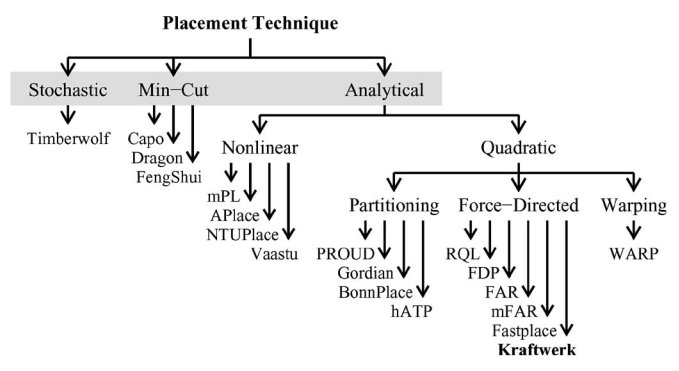
\includegraphics[width=0.75\textwidth]{figures/kraftwerk2.png}
            \end{center}
            \caption{Landscape of VLSI placement techniques (Spindler) \cite{kraftwerk2} }
            \label{fig:}
        \end{figure}
        \begin{figure}
            \begin{center}
                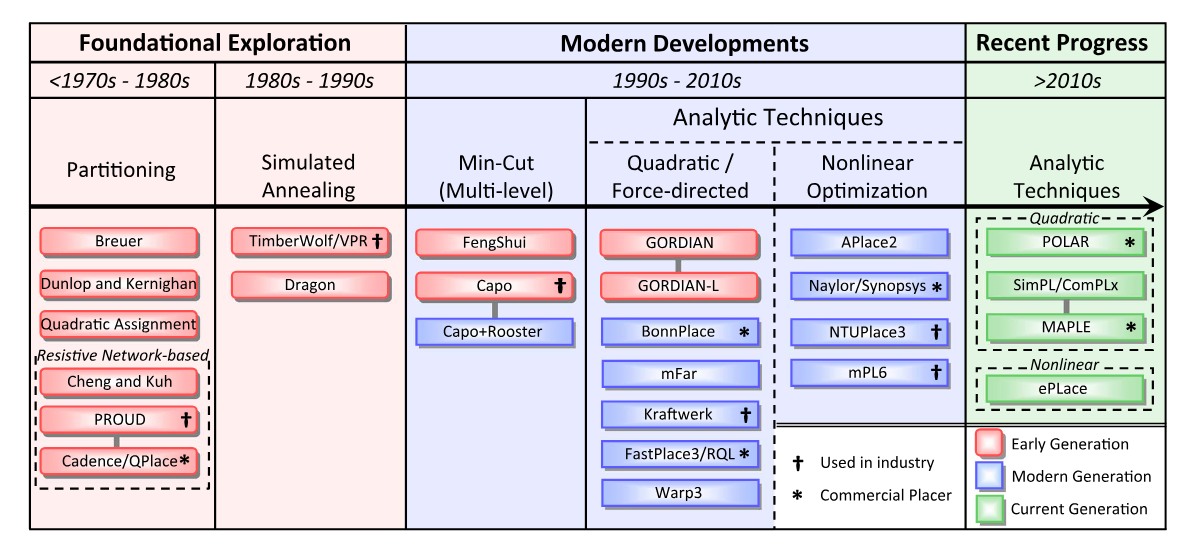
\includegraphics[width=0.95\textwidth]{figures/ProCha.png}
            \end{center}
            \caption{Historical timeline of VLSI placement techniques (Markov) \cite{ProCha} }
            \label{fig:}
        \end{figure}
    \end{itemize}

\end{itemize}

This is a citation for AMFPlacer. \cite{AMFPlacer}

\newpage
\bibliographystyle{ieeetr}
\nocite{*}
\bibliography{
    references/surveys,
    references/rapidwright,
    references/fpga_placement,
    references/vlsi_placement,
}

\end{document}


